\documentclass[../psets.tex]{subfiles}

\pagestyle{main}
\renewcommand{\leftmark}{Problem Set \thesection}
\setcounter{section}{2}

\begin{document}




\section{Noncovalent Interactions and Thermodynamics}
\marginnote{11/14:}The questions pertain to the material covered from Noncovalent Interactions (Oct 24) to Isotope Effects (Nov 5).
\begin{enumerate}
    \item The $\pi$-$\pi$ interaction in aromatic systems plays an important role in the fields of chemistry and biology. It affects the crystal packing of organic molecules, molecular recognition processes, and the three-dimensional structures of proteins and DNA.
    \begin{enumerate}
        \item Please use Rowan to complete this question.
        \begin{enumerate}
            \item Using any means, build a molecular model for benzene in Rowan. Then, perform a geometry optimization and charge calculation using the r\textsuperscript{2}SCAN-3c method. Take a screenshot of the webpage before submitting the job and paste it here.
            \begin{itemize}
                \item Note: this job should not take more than 1 minute to run (not including queue time). If
                it takes significantly longer, consider adjusting your initial bond lengths/angles.
            \end{itemize}
            \begin{proof}
                {\color{white}hi}
                \begin{center}
                    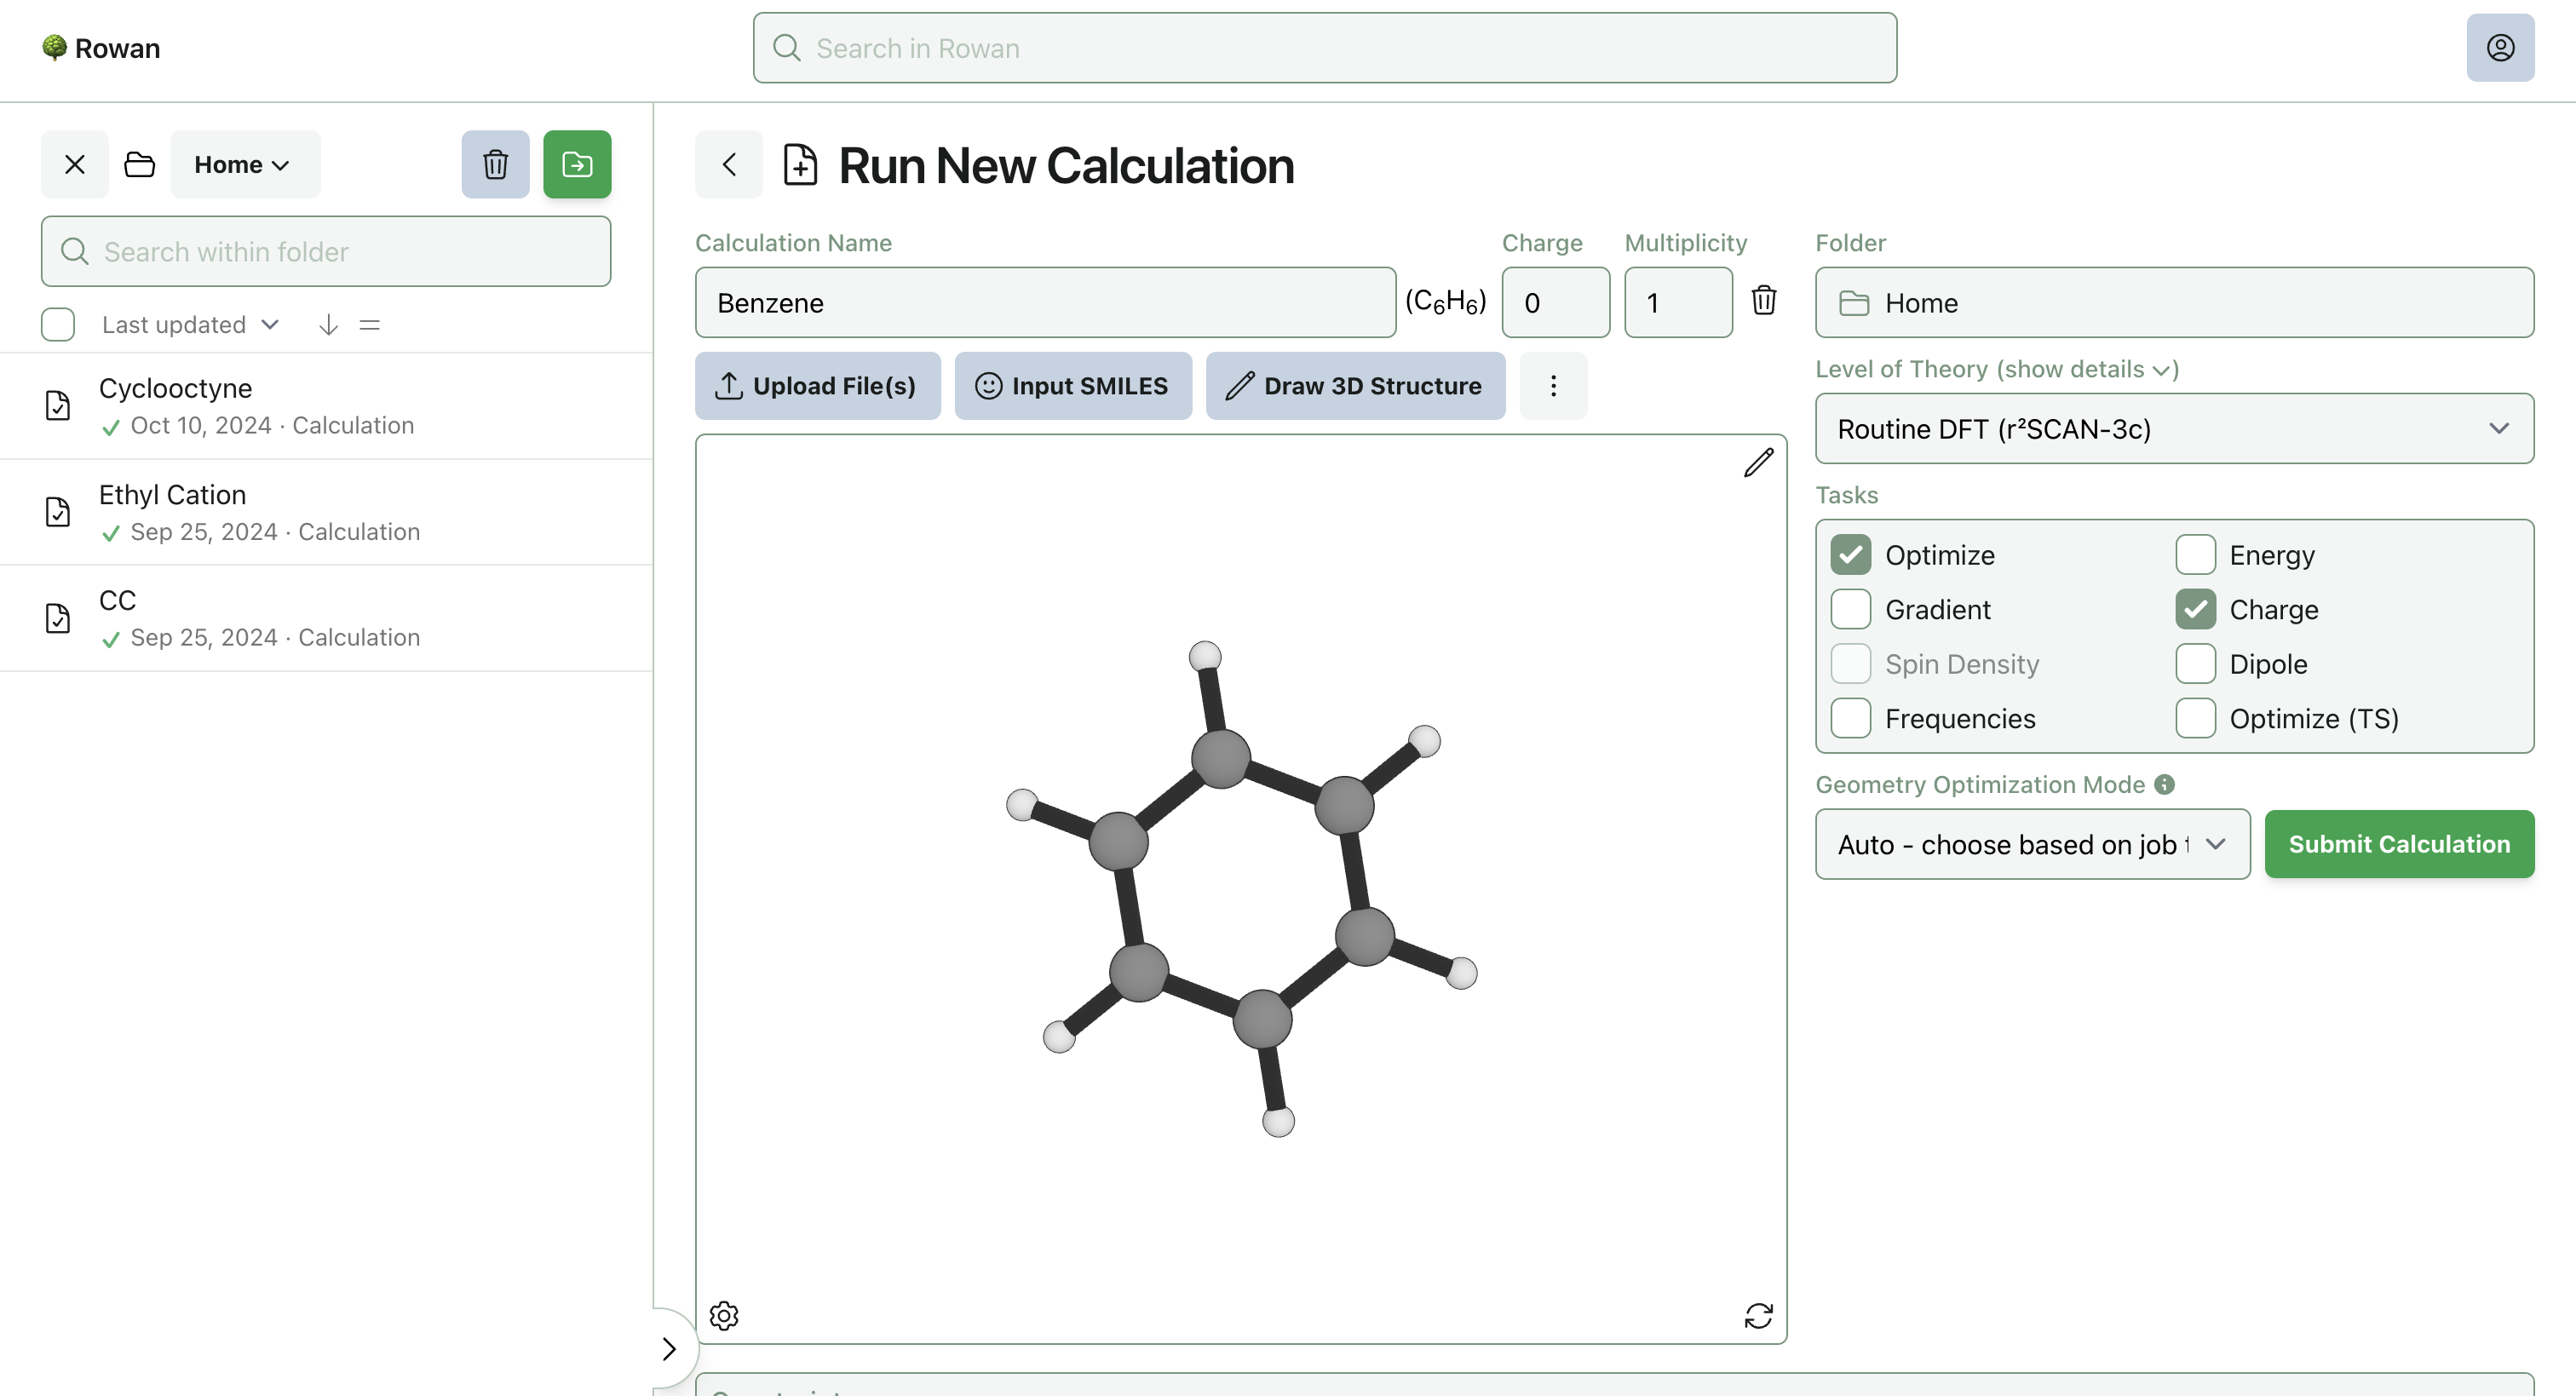
\includegraphics[width=0.9\linewidth]{PSet3Q1ai.png}
                \end{center}
            \end{proof}
            \item Convert the optimized structure into cartesian (XYZ) coordinates and paste them here.
            \begin{proof}
                {\color{white}hi}\\
                C     1.08186398   0.87624363  -0.02492904\\
                C     1.29957353  -0.49892653  -0.02069362\\
                C     0.21782415  -1.37512819   0.00423309\\
                C    -1.08186402  -0.87624412   0.02492904\\
                C    -1.29957346   0.49892716   0.02069361\\
                C    -0.21782322   1.37512844  -0.00423311\\
                H     1.92529173   1.55932611  -0.04436360\\
                H     2.31283908  -0.88800382  -0.03682784\\
                H     0.38774005  -2.44726076   0.00753188\\
                H    -1.92529254  -1.55932713   0.04436366\\
                H    -2.31283985   0.88800436   0.03682783\\
                H    -0.38773950   2.44726073  -0.00753189\\
            \end{proof}
            \item How are the charges distributed on the molecule?
            \begin{proof}
                The Mulliken partial charges are all concentrated symmetrically on the carbon atoms, $-0.150$ on each carbon and $+0.150$ on each hydrogen.
            \end{proof}
        \end{enumerate}
        \pagebreak
        \item As mentioned in class, benzene rings can interact through various geometries. Explain why the displaced and T-shaped configurations may exhibit lower energies compared to the sandwich geometry. In your discussion, include considerations of polarization effects and electrostatic interactions.
        \begin{center}
            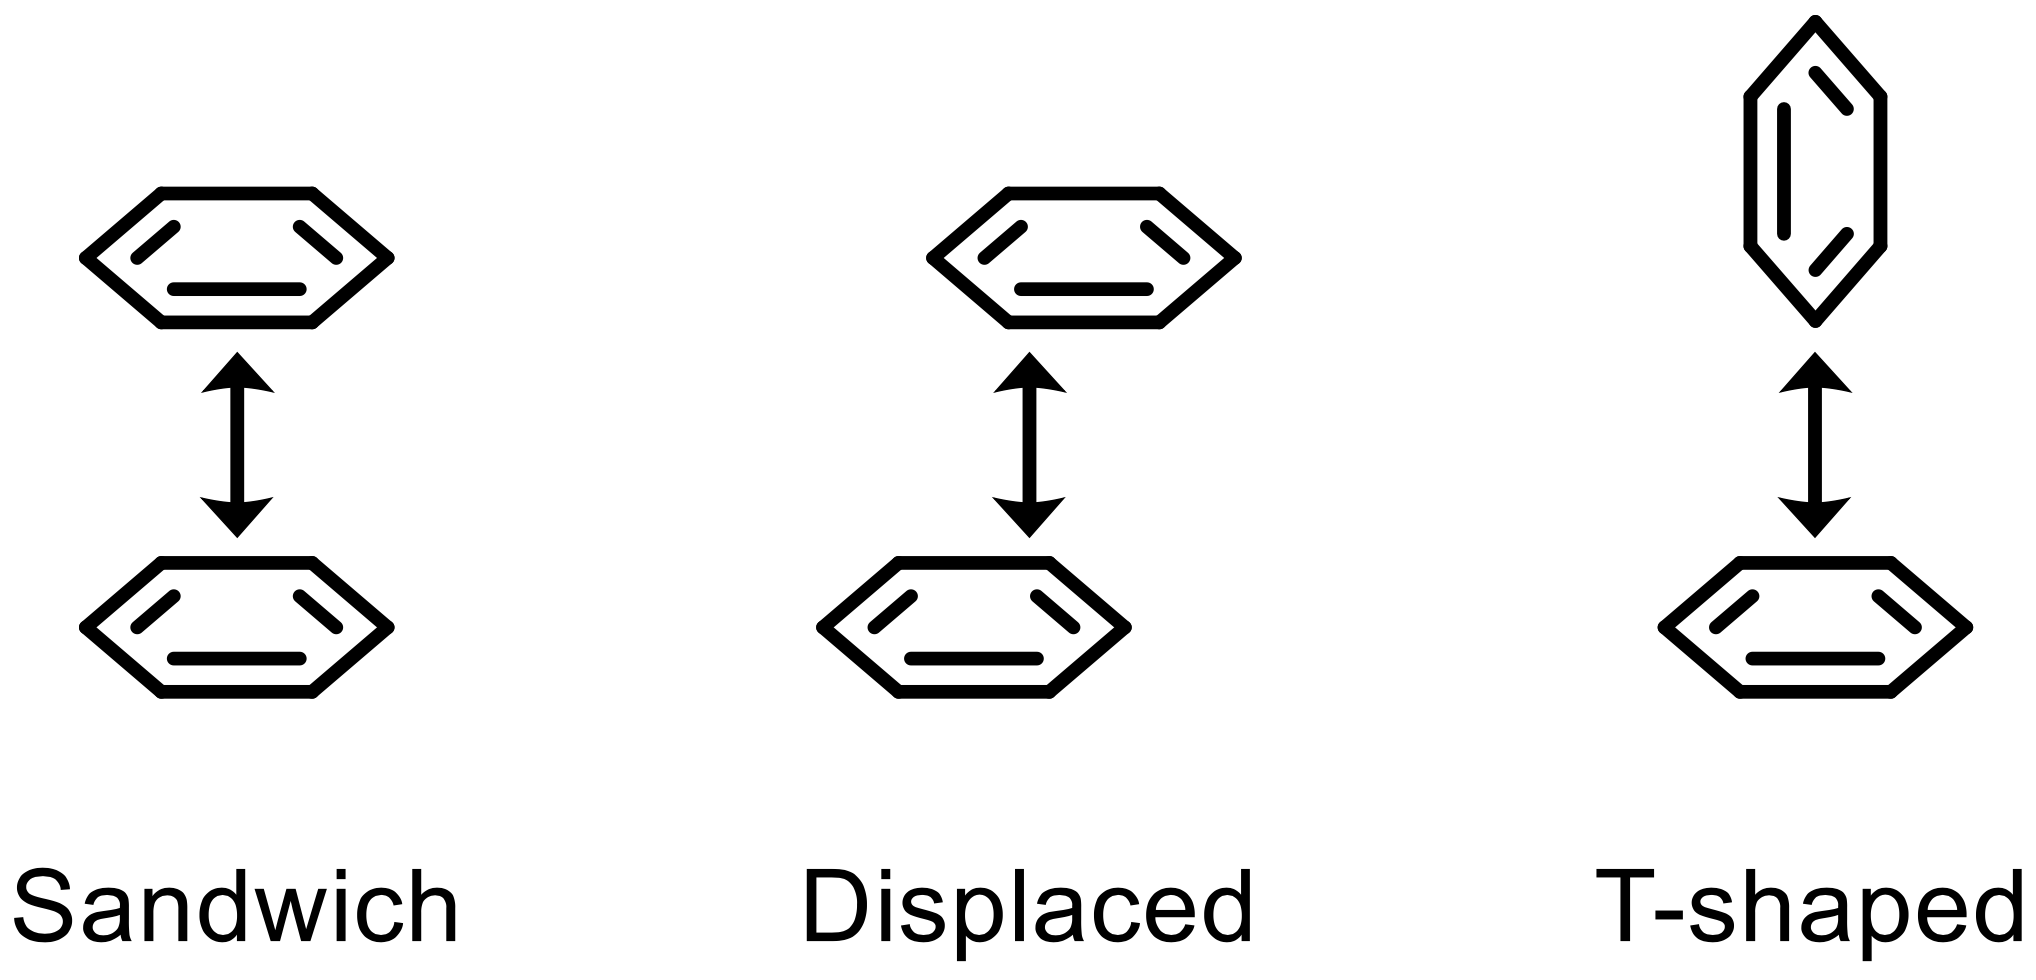
\includegraphics[width=0.4\linewidth]{PSet3F1.png}
        \end{center}
        \begin{proof}
            It is more favorable for benzene rings to interact through quadrupole-type noncovalent interactions. In sandwich stacking, two regions of negative charge touch each other. On the other hand, in both displaced and T-shaped stacking, a region of partial negative charge (the center of the ring) can interact with a region of partial positive charge (the edge of another ring).
        \end{proof}
    \end{enumerate}
    \pagebreak
    \item The reaction of dichlorocarbene with isobutylene is known to be one of the exceptions where the reaction has a negative activation enthalpy ($\Delta H^\ddagger$).
    \begin{center}
        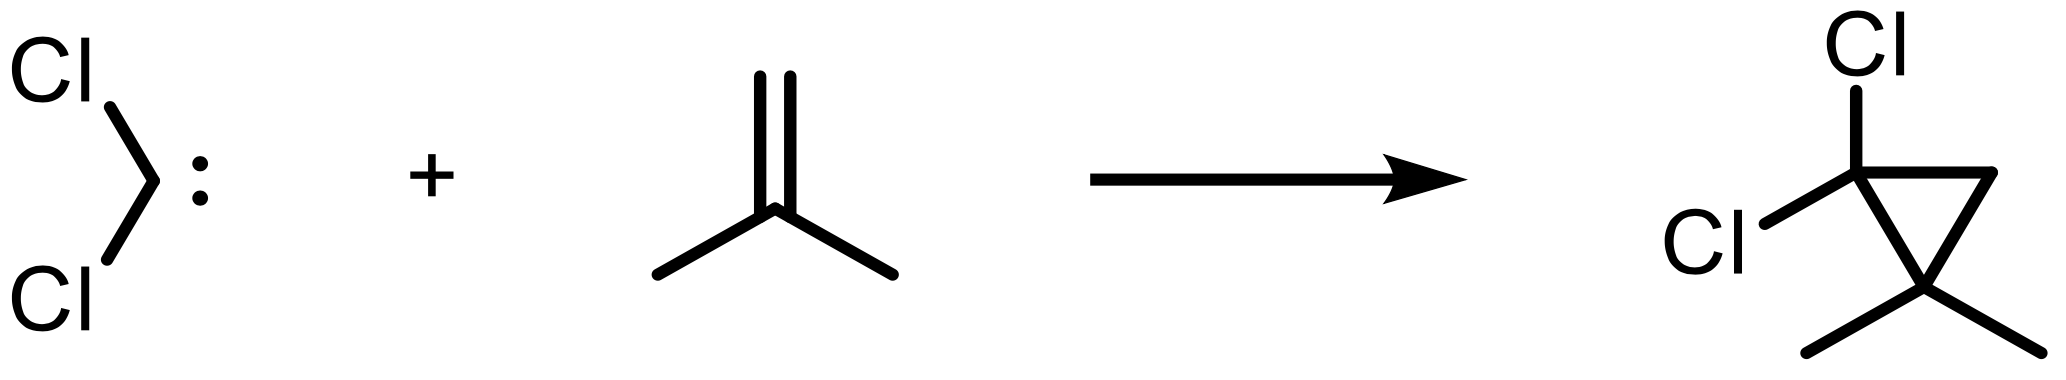
\includegraphics[width=0.4\linewidth]{PSet3F2.png}
    \end{center}
    \begin{enumerate}
        \item Consider the reverse reaction. Conduct a thought experiment in which we gradually pull dichlorocarbene away from isobutylene. How would $\Delta H$ vary with distance? How would $\Delta S$ vary with distance? Draw an energy diagram depicting both $\Delta H$ and $-T\Delta S$ as functions of distance on a single plot. Assume that $\Delta H$ and $\Delta S$ are zero at infinite distance.
        \begin{proof}
            The forward reaction proceeds via a side-to-side interaction of either the carbene HOMO and alkene LUMO, or the carbene LUMO and alkene HOMO. Without the loss of generality, let's consider the case of the carbene HOMO and alkene LUMO. As these orbitals mix, we get enthalpically favorable steric stabilization like in the silylene example from the 10/24  NCIs lecture.\par
            Thus, considering the reverse reaction, entering higher vibrational states of the two `new' \ce{C-C} bonds eventually leads to the two species eventually "pinging" apart, as in the \ce{{}^{\emph{t}}Bu-Cl} example from the 10/29 equilibria lecture. As we pull apart the `starting materials,' we consistently decrease orbital mixing, which is consistently enthalpically disfavorable; we do not later get any type of favorable process such as solvation.\par
            Thus, $\Delta H$ varies with distance ($d$) by decreasing from zero at $d=\infty$ to the product bond length, and then increasing to some finite (not infinite) value. So the potential is vaguely Lennard-Jones like, in that attraction gets more favorable when the distance gets closer, up to the point when the carbene nucleus starts getting too close to the alkene nuclei. However, it never goes to $\infty$ because --- unlike in the \ce{{}^{\emph{t}}BuCl} example --- $d=0$ does \emph{not} correspond to two nuclei being on top of each other, which would be infinite energy.\par
            $-T\Delta S$ increases as distance decreases, accelerating as the species get closer together. This is because the entropy drops as we go from two molecules to one, probably by close to \eu{30}. Essentially, we are forming a highly-ordered single-molecule product that is much less entropically favorable.
            \begin{center}
                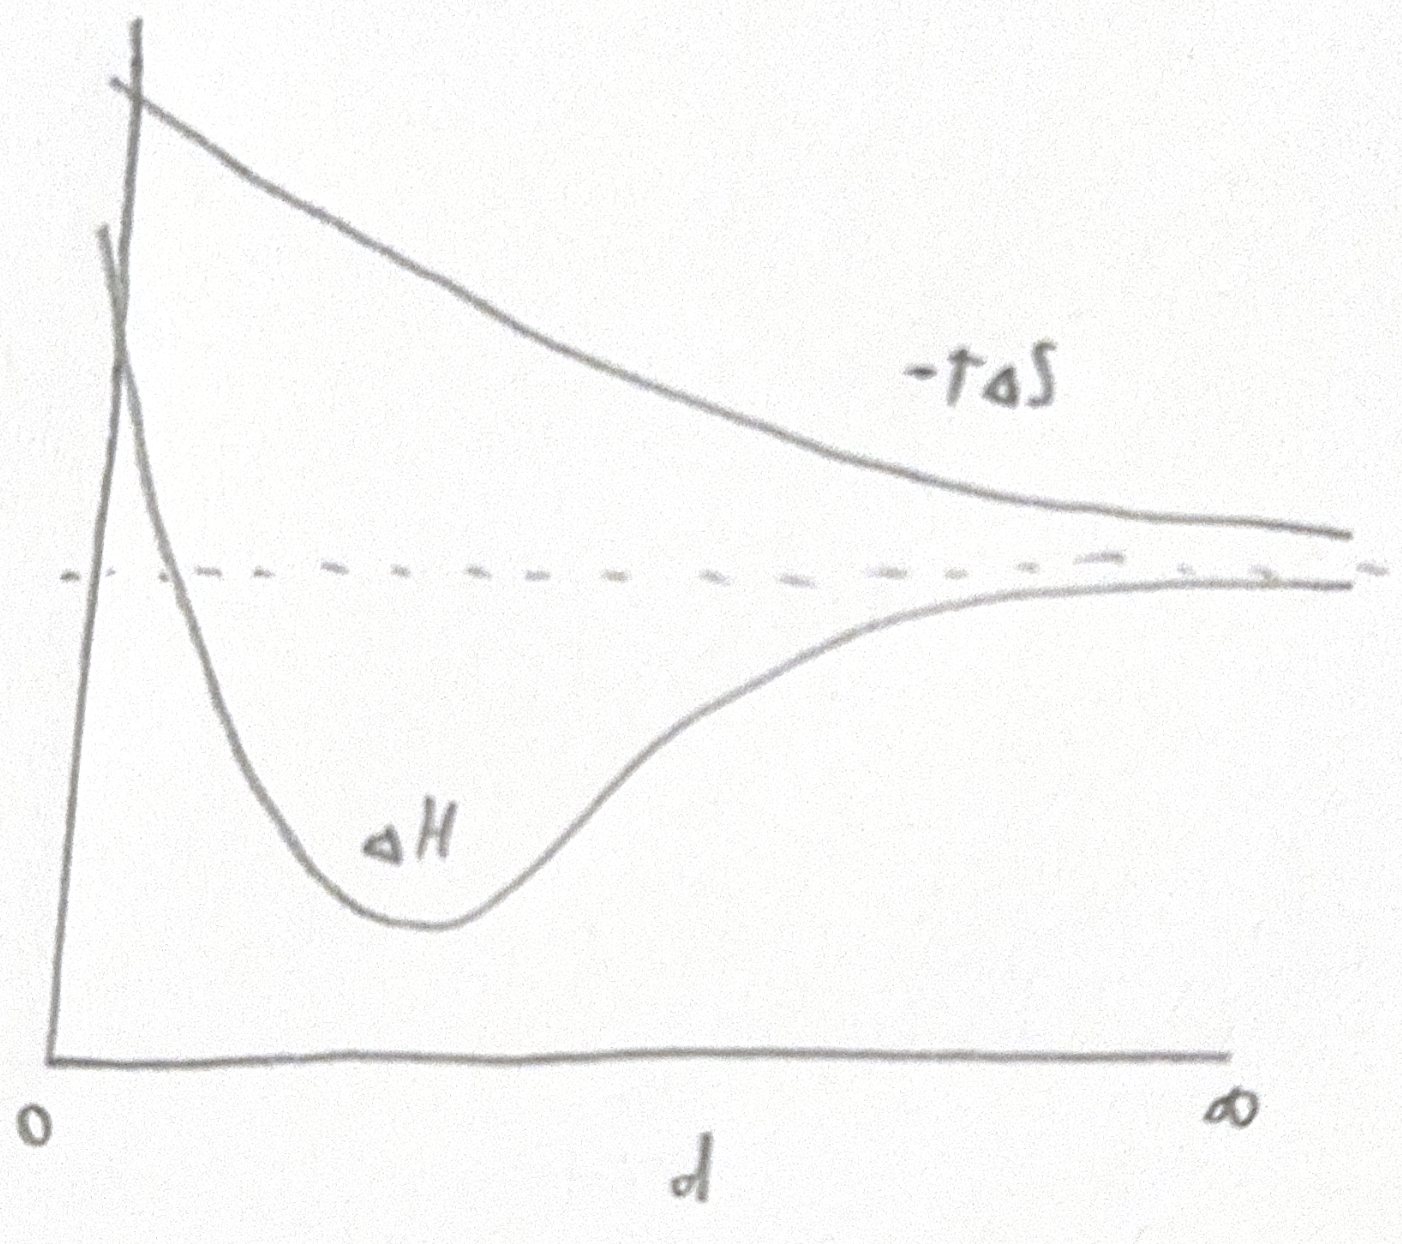
\includegraphics[width=0.5\linewidth]{PSet3Q2a.png}
            \end{center}
        \end{proof}
        \pagebreak
        \item If $\Delta H$ dominates at a short distance, and $\Delta S$ dominates at a large distance between the molecules, how would $\Delta G$ change as a function of distance? Draw an energy diagram for $\Delta G$ on the plot from part (a).
        \begin{proof}
            As the molecules get farther apart, $\Delta G$ would be negative at first (due to $\Delta H$) and then positive later (due to $\Delta S$).
            \begin{center}
                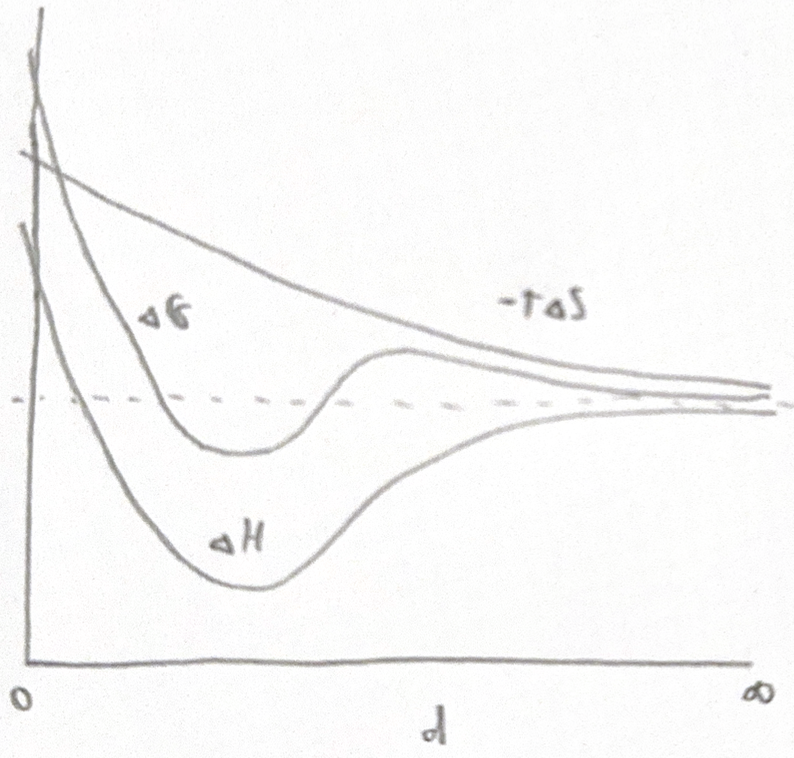
\includegraphics[width=0.5\linewidth]{PSet3Q2b.png}
            \end{center}
        \end{proof}
        \item Indicate $\Delta G^\ddagger$, $\Delta H^\ddagger$, and $T\Delta S^\ddagger$ on the diagram and explain why this reaction exhibits a negative activation enthalpy.
        \begin{proof}
            {\color{white}hi}
            \begin{center}
                \includegraphics[width=0.5\linewidth]{PSet3Q2c.png}
            \end{center}
            By definition, the activated complex is the highest energy point on the potential \emph{energy} surface along the reaction coordinate. Thus, I have drawn all three arrows at the peak in $\Delta G$.\par
            The reaction exhibits a negative activation enthalpy because at the activated complex, the change in enthalpy $\Delta H^\ddagger$ from separate species ($\Delta H^\ddagger=0$ at $d=\infty$) is negative.
        \end{proof}
    \end{enumerate}
    \pagebreak
    \item The following table presents the experimentally measured kinetic data for a Diels-Alder reaction between tetracyanoethylene (TCNE) and 9,10-dimethylanthracene (DMA).
    \begin{center}
        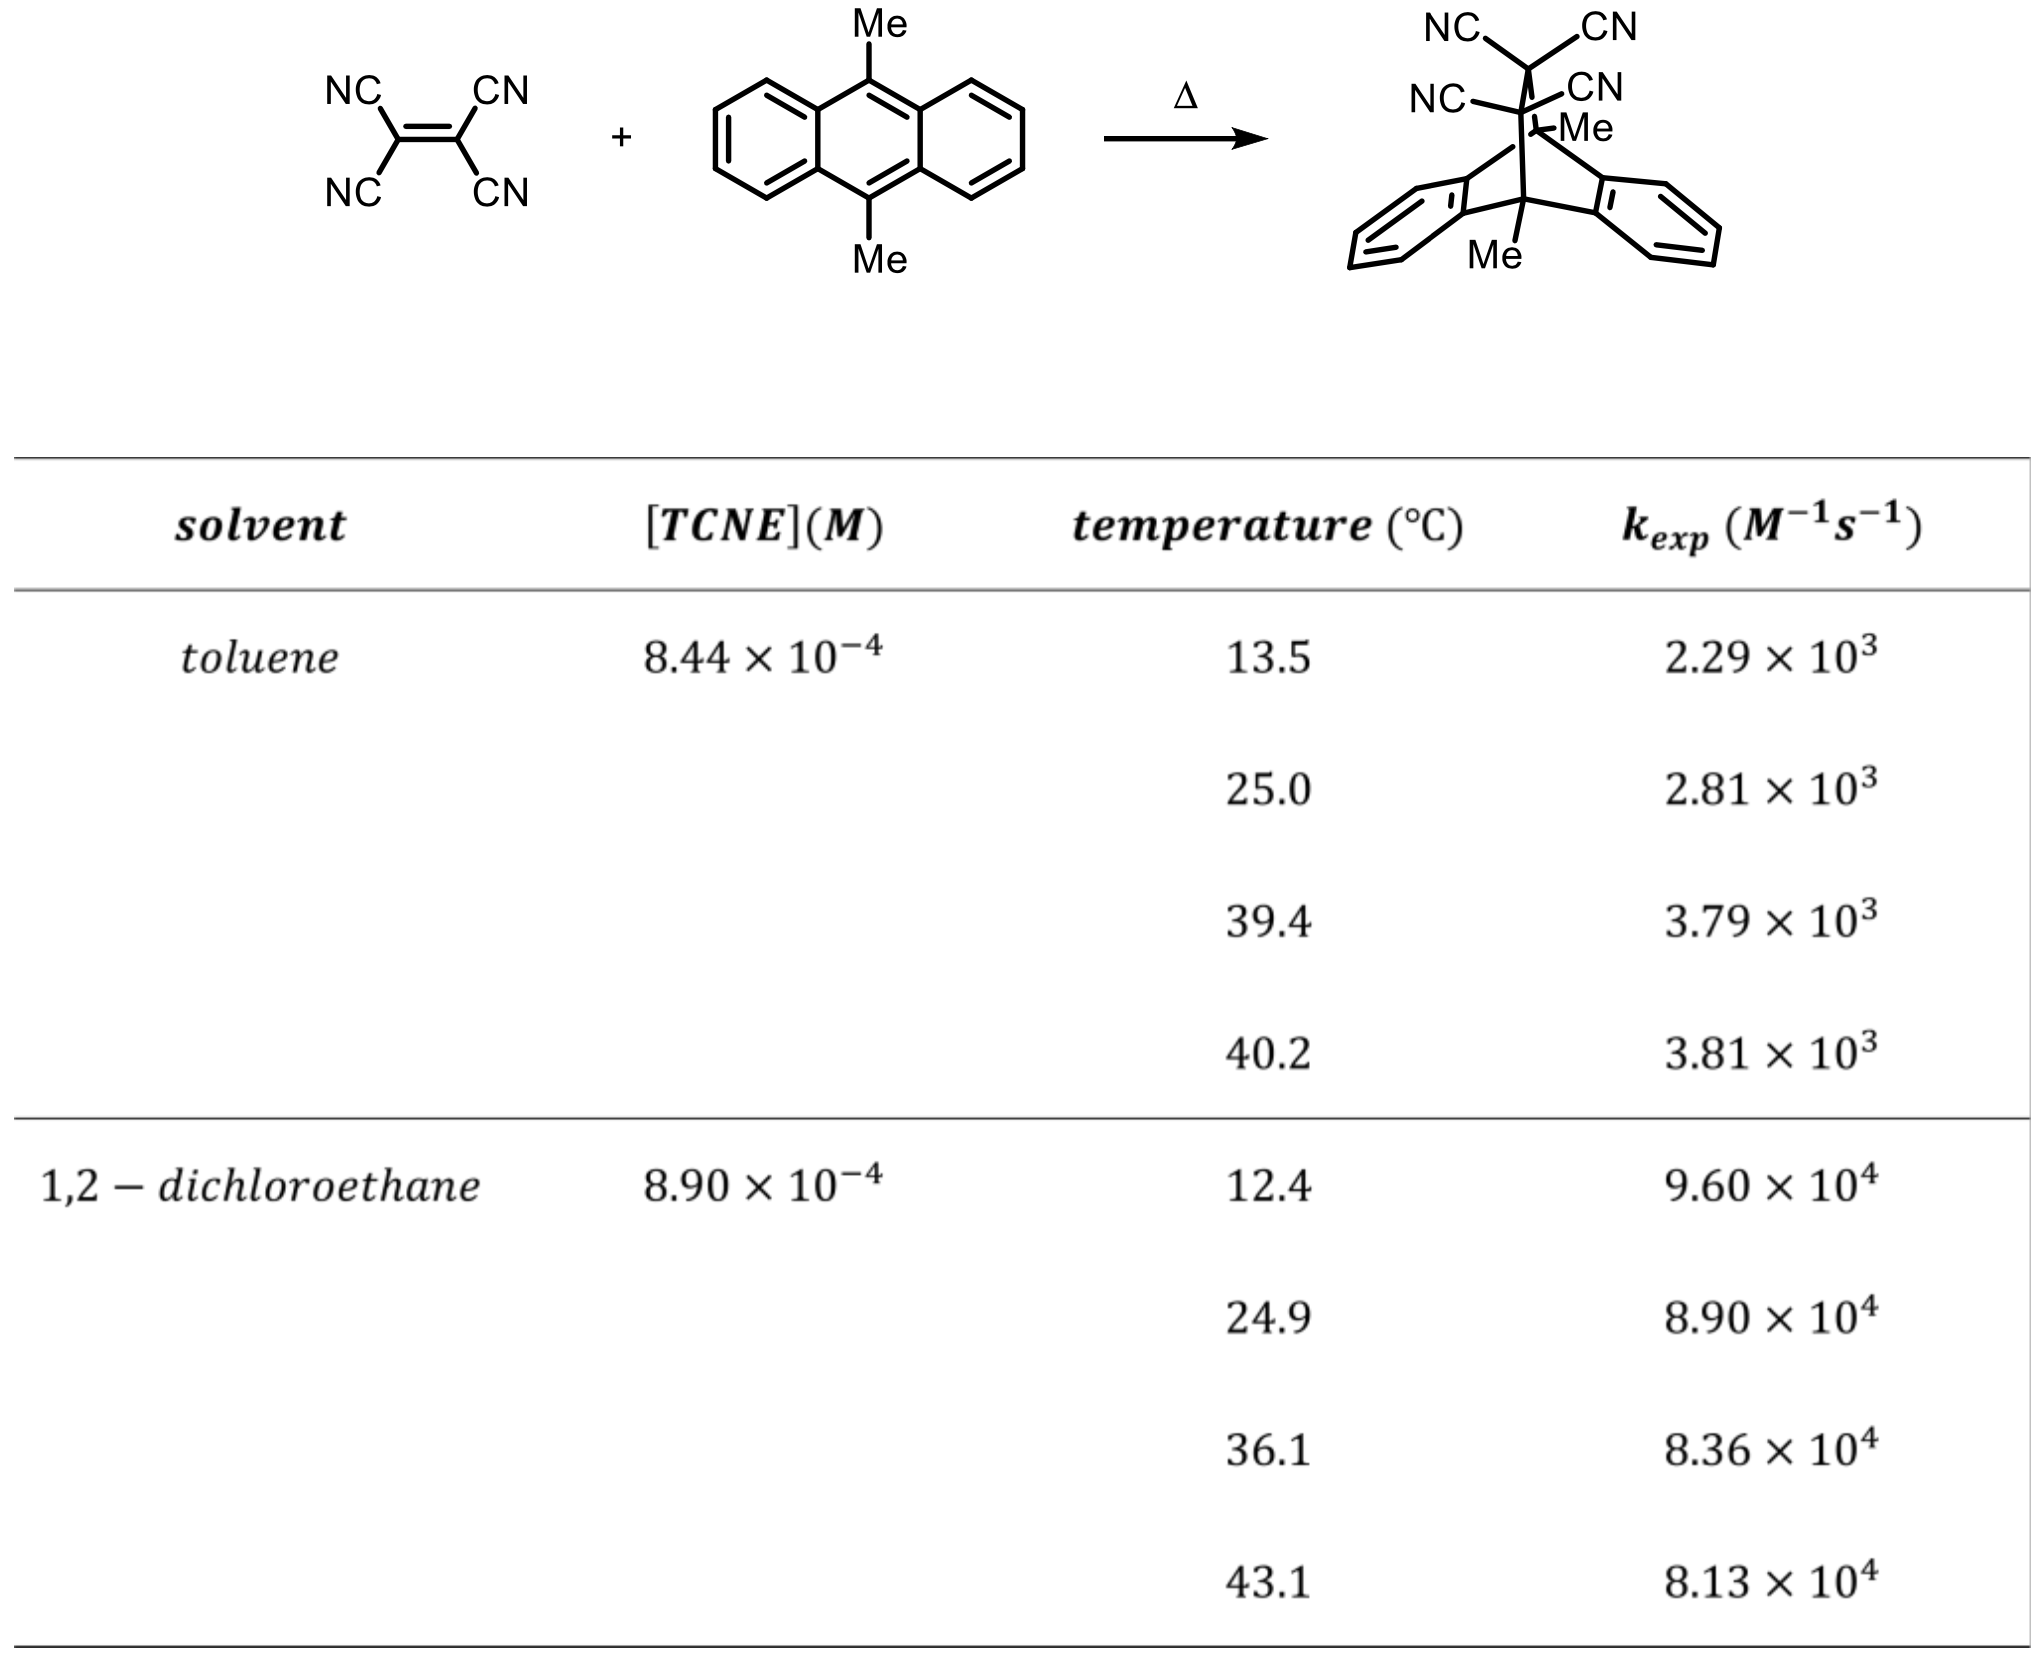
\includegraphics[width=0.8\linewidth]{PSet3F3.png}
    \end{center}
    \begin{enumerate}
        \item Use this data to determine the observed activation enthalpy ($\Delta H^\ddagger$) and activation entropy ($\Delta S^\ddagger$) for the reaction in the following solvents. Use Excel or a similar program to answer the question, and give your answers in units of \si{\kilo\calorie\per\mole} and/or \si{\entropyunit} (\si{\calorie\per\kelvin\per\mole}).
        \begin{enumerate}
            \item Toluene.
            \begin{proof}
                To solve for $\Delta H^\ddagger$ and $\Delta S^\ddagger$ using experimental temperature-rate constant data, we will use an Eyring plot. This method works off of the following linearization of the Eyring equation
                \begin{equation*}
                    \ln(\frac{kh}{\kappa\kB T}) = -\frac{\Delta H^\ddagger}{R}\left( \frac{1}{T} \right)+\frac{\Delta S^\ddagger}{R}
                \end{equation*}
                where $k=k_\text{exp}$, $h=\SI{6.626e-34}{\joule\second}$ is Planck's constant in the appropriate units, $\kappa$ is the transmission coefficient, $\kB=\SI{1.381e-23}{\joule\per\kelvin}$ is the Boltzmann constant, $T$ is the temperature in Kelvin, and $R=\SI{1.9872e-3}{\kilo\calorie\per\mole\per\kelvin}=\eu{1.9872}$ is the ideal gas constant. In accordance with the second fundamental assumption of transition state theory --- that any molecule that makes its way to the transition state will then proceed onto the product barrierlessly --- we choose $\kappa=1$. Thus, our raw temperature-rate constant data become
                \begin{center}
                    \small
                    \renewcommand{\arraystretch}{1.2}
                    \begin{tabular}{c|c}
                        $\bm{1/T}$ $(\textbf{K}^{-1})$ & $\bm{\textbf{ln}(kh/k_\textbf{B}T)}$\\
                        \hline
                        \num{3.49e-3} & $-21.682$\\
                        \num{3.35e-3} & $-21.517$\\
                        \num{3.20e-3} & $-21.265$\\
                        \num{3.19e-3} & $-21.262$\\
                    \end{tabular}
                \end{center}
                Performing a linear regression, we can determine that
                \begin{align*}
                    -\frac{\Delta H^\ddagger}{R} &= -\SI{1440}{\kelvin}&
                    \frac{\Delta S^\ddagger}{R} &= -16.7\\
                    \Aboxed{\Delta H^\ddagger &= \kcal{2.86}}&
                    \Aboxed{\Delta S^\ddagger &= -\eu{33.2}}
                \end{align*}
            \end{proof}
            \item 1,2-dichloroethane.
            \begin{proof}
                Apply an analogous technique to Q1ai: Start by manipulating the data
                \begin{center}
                    \small
                    \renewcommand{\arraystretch}{1.2}
                    \begin{tabular}{c|c}
                        $\bm{1/T}$ $(\textbf{K}^{-1})$ & $\bm{\textbf{ln}(kh/k_\textbf{B}T)}$\\
                        \hline
                        \num{3.50e-3} & $-17.943$\\
                        \num{3.36e-3} & $-18.061$\\
                        \num{3.23e-3} & $-18.161$\\
                        \num{3.16e-3} & $-18.211$\\
                    \end{tabular}
                \end{center}
                and then perform a linear regression
                \begin{align*}
                    -\frac{\Delta H^\ddagger}{R} &= \SI{789}{\kelvin}&
                    \frac{\Delta S^\ddagger}{R} &= -20.7\\
                    \Aboxed{\Delta H^\ddagger &= -\kcal{1.57}}&
                    \Aboxed{\Delta S^\ddagger &= -\eu{41.1}}
                \end{align*}
            \end{proof}
        \end{enumerate}
        \item Considering that $\Delta H^\ddagger$ is positive for most reactions, what is notable about the observed $\Delta H^\ddagger$ value(s) in the above case(s)?
        \begin{proof}
            When the reaction is run in 1,2-dichloroethane, there are is a \emph{negative} enthalpy of activation as in Q2.
        \end{proof}
        \item Both experiments and theory support the existence of an intermediate between the starting materials and the product in this reaction, known as an electron donor-acceptor molecular complex. Draw a potential energy diagram with $\Delta H$ (change in enthalpy) on the $y$-axis to rationalize the observed abnormality in part (b).
        \begin{proof}
            {\color{white}hi}
            \begin{center}
                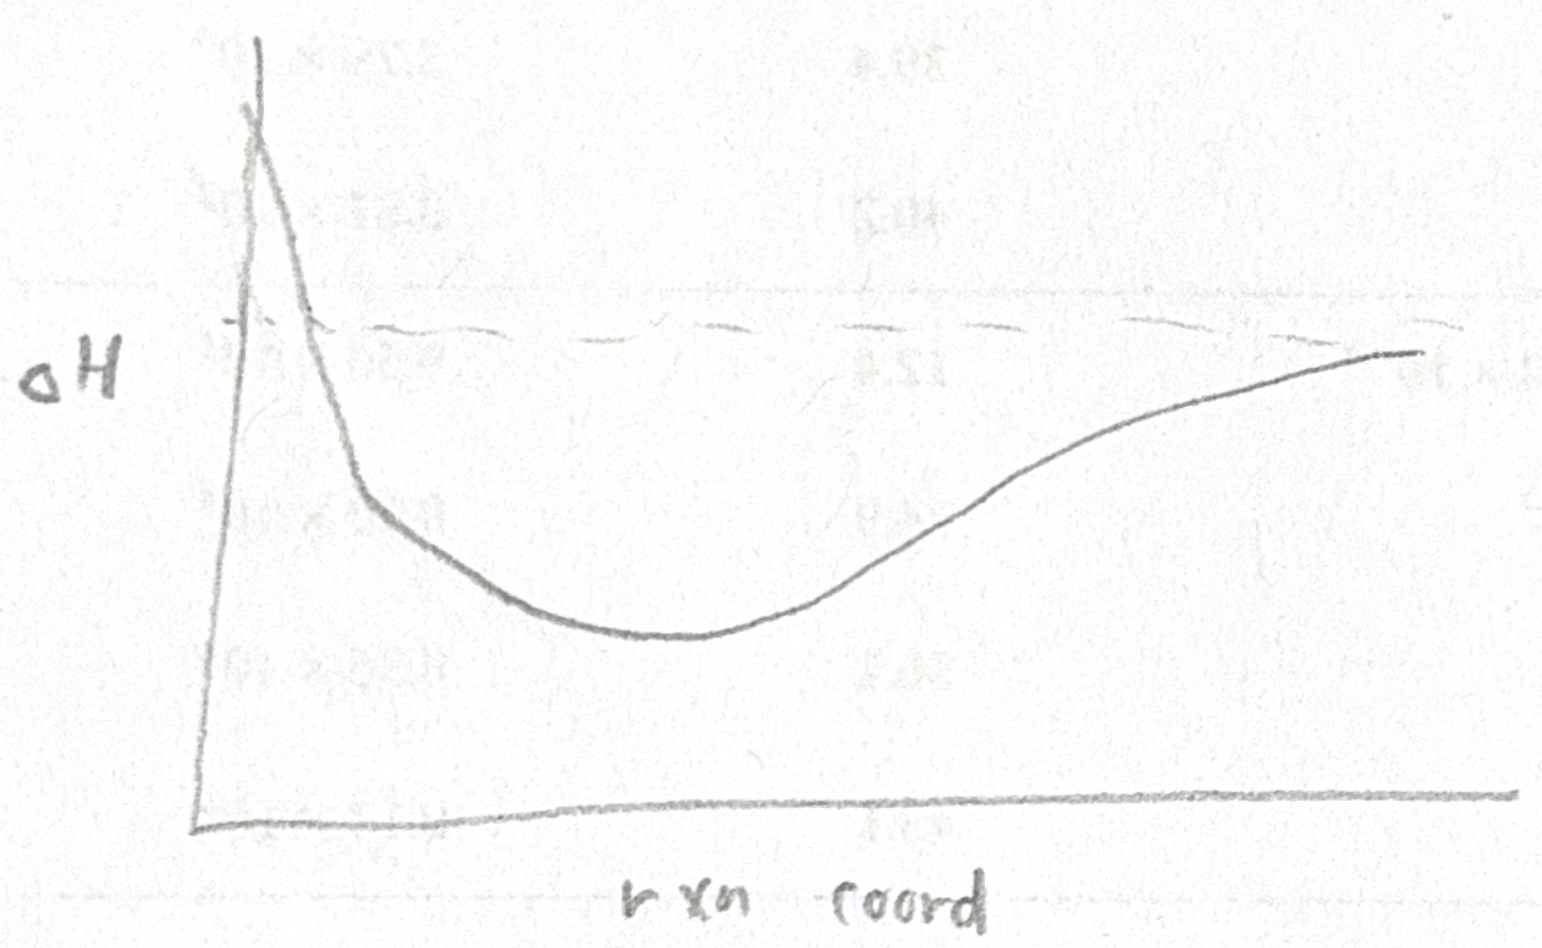
\includegraphics[width=0.5\linewidth]{PSet3Q3c.png}
            \end{center}
            Due to the existence of a stable intermediate, this reaction can have a negative $\Delta H^\ddagger$.
        \end{proof}
        \pagebreak
        \item The mechanism of this reaction is known to be the same in toluene and 1,2-dichloroethane. Based on your answers from part (a) and your energy diagram from part (c), explain how the solvent can make a difference in observed $\Delta H^\ddagger$.
        \begin{proof}
            The solvent can affect the stability of the intermediate and the height of the barrier between intermediate \ce{I} and the product \ce{P}. Relatively polar 1,2-dichloroethane is more likely to stabilize the polar intermediate and the transition state, thereby resulting in a negative activation enthalpy for the overall reaction.
        \end{proof}
    \end{enumerate}
    \pagebreak
    \item Beak has reported an example of `dynamic thermodynamic resolution' in the asymmetric silylation of benzylic carbanions. In this work, a racemic mixture of dianion \textbf{1} is ligated with 1 equivalent of enantiopure amine \textbf{2} at $-\SI{78}{\celsius}$ to form equal amounts of two new diastereomeric amine-lithium complexes (\textbf{3} and $\bm{3'}$) that have unequal energy. Although the \ce{C-Li} stereocenter in \textbf{3} and $\bm{3'}$ is configurationally stable at $-\SI{78}{\celsius}$, upon warming to $-\SI{25}{\celsius}$, these two complexes readily equilibrate. Upon cooling back to $-\SI{78}{\celsius}$, these anions both react stereospecifically with trimethylsilyl chloride (\ce{TMSCl}) to form enantiomeric products \textbf{4} and $\bm{4'}$. Use this description and the data provided below to answer the following questions. (Equivalents of \ce{TMSCl} are with respect to \textbf{1}).
    \begin{center}
        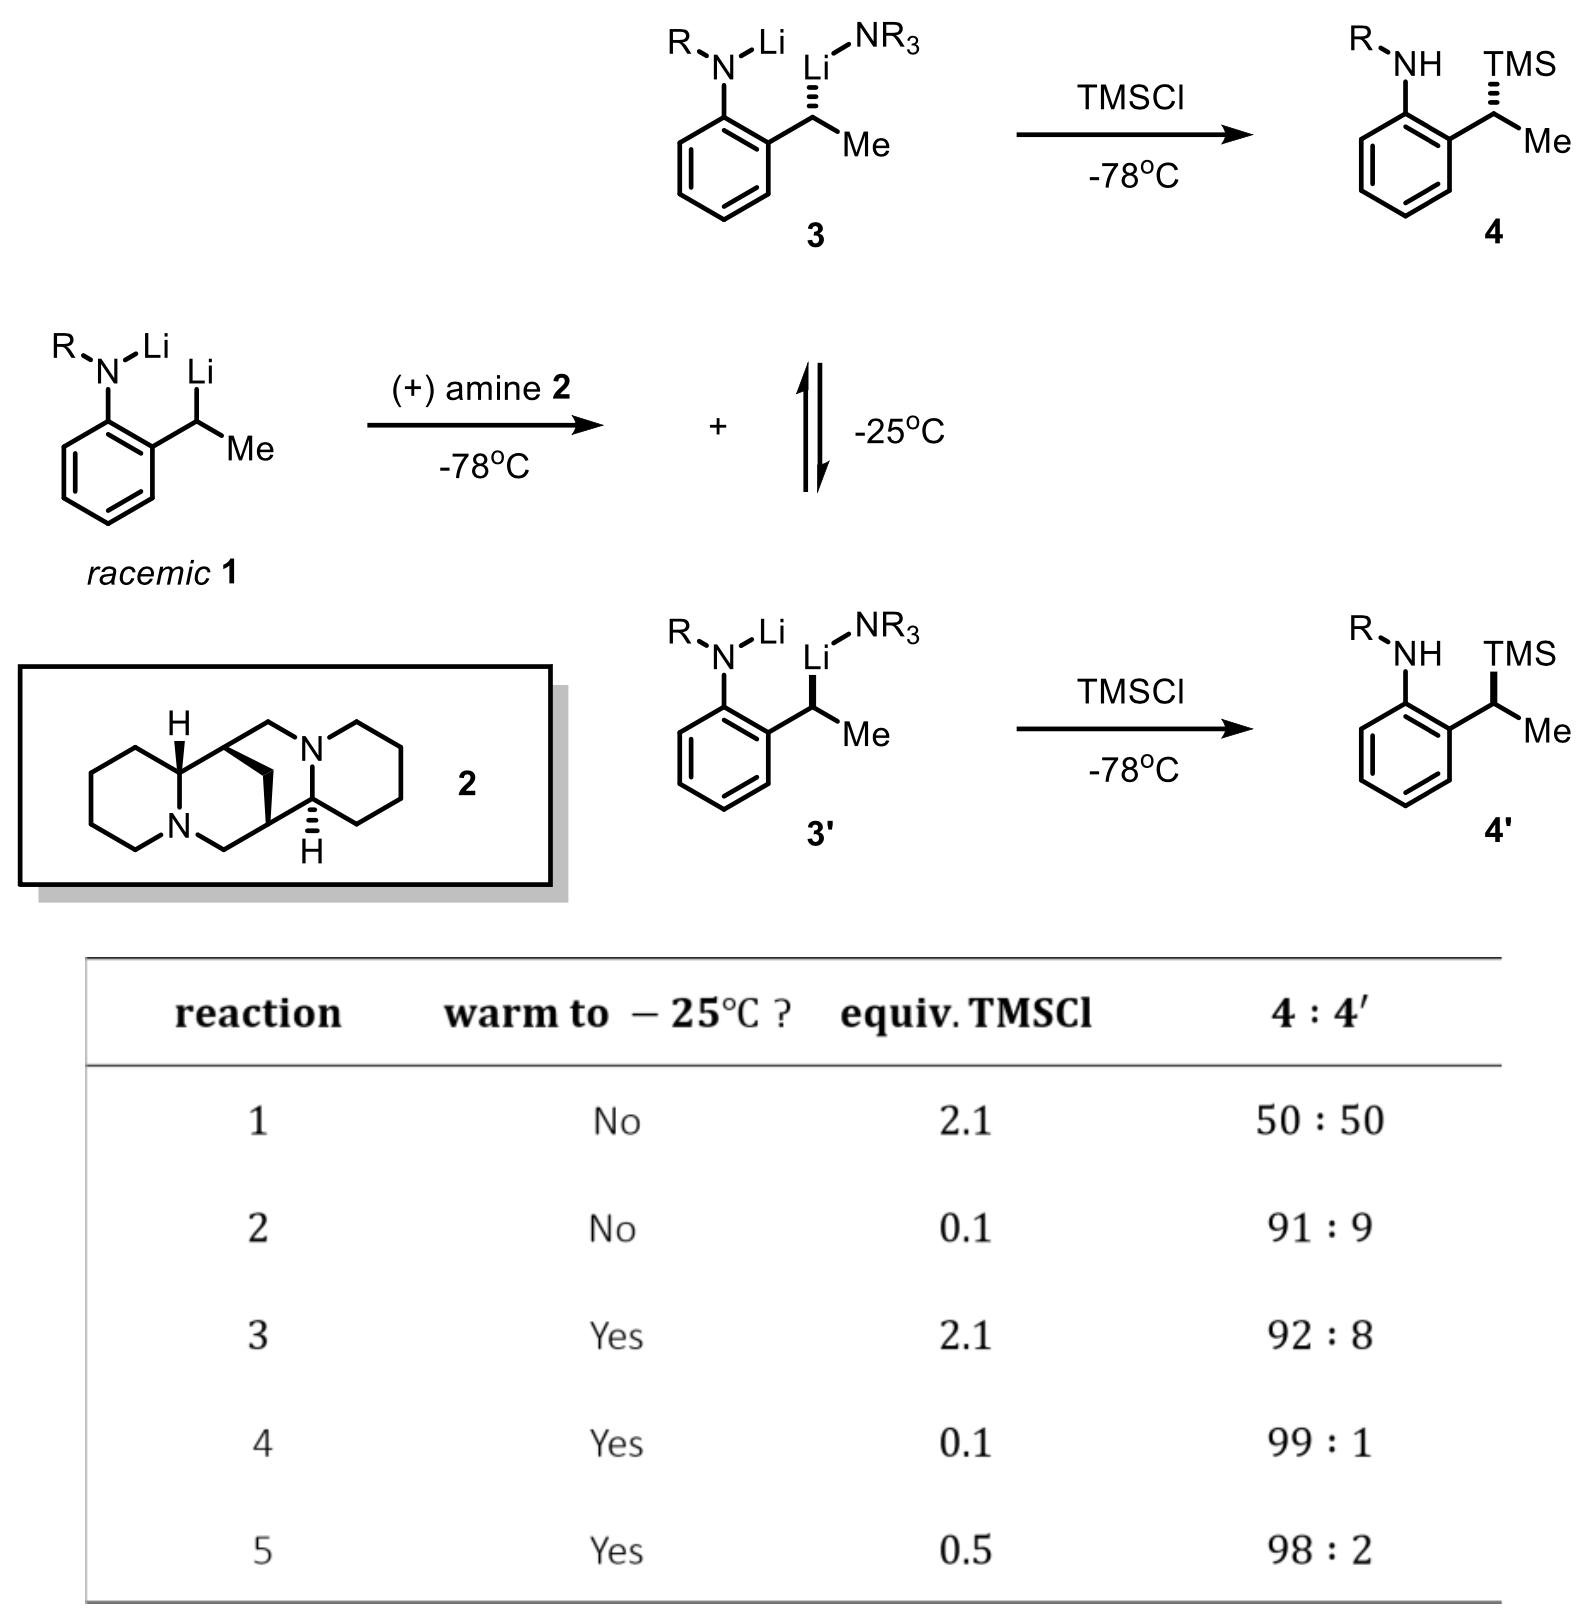
\includegraphics[width=0.8\linewidth]{PSet3F4.png}
    \end{center}
    \begin{enumerate}
        \item Calculate $\Delta G^\circ$ for \textbf{3} and $\bm{3'}$ at $-\SI{25}{\celsius}$.
        \begin{proof}
            Reaction 3 has excess \ce{TMSCl}, so we get quantitative conversion of \textbf{3} to \textbf{4} and $\bm{3'}$ to $\bm{4'}$. Thus, the equilibrium ratio of \textbf{3} to $\bm{3'}$ is $92:8$! It follows that
            \begin{equation*}
                \Keq = \frac{8}{92}
            \end{equation*}
            and hence
            \begin{align*}
                \Delta G^\circ &= -RT\ln\Keq\\
                &= -\left( \SI[per-mode=fraction]{1.9872e-3}{\kilo\calorie\per\mole\per\kelvin} \right)\left( \SI{248}{\kelvin} \right)\ln(\frac{8}{92})\\
                \Aboxed{\Delta G^\circ &= \kcal{1.2}}
            \end{align*}
        \end{proof}
        \item Calculate $\Delta\Delta G^\ddagger$, for the reactions of \textbf{3} and $\bm{3'}$ with \ce{TMSCl} at $-\SI{78}{\celsius}$.
        \begin{proof}
            In reality, the kinetics of the reactions of \textbf{3} and $\bm{3'}$ with \ce{TMSCl} are governed by the following system of coupled nonlinear ordinary differential equations.
            \begin{align*}
                -\dv{[\bm{3}]}{t}  &= k_{\bm{34}}[\bm{3}]\cnc{TMSCl}&
                -\dv{[\bm{3'}]}{t} &= k_{\bm{3'4'}}[\bm{3'}]\cnc{TMSCl}
            \end{align*}
            There is no analytical solution to these rate laws. However, under \emph{low} conversion from equal amounts of starting materials, the product ratio is \emph{approximately} equal to the $k$ ratio since we're \emph{closer} to observing initial rates:
            \begin{equation*}
                \frac{k_{\bm{34}}}{k_{\bm{3'4'}}} \approx \frac{[\bm{4}]}{[\bm{4'}]}
            \end{equation*}
            Thus, using Reaction 2 as our proxy for low conversion with equal amounts of \textbf{3} and $\bm{3'}$, we have
            \begin{align*}
                \Delta\Delta G^\ddagger &= -RT\ln(\frac{k_{\bm{34}}}{k_{\bm{3'4'}}})\\
                &= -RT\ln(\frac{[\bm{4}]}{[\bm{4'}]})\\
                &= -\left( \SI[per-mode=fraction]{1.9872e-3}{\kilo\calorie\per\mole\per\kelvin} \right)\left( \SI{195}{\kelvin} \right)\ln(\frac{91}{9})\\
                \Aboxed{\Delta\Delta G^\ddagger &= -\kcal{0.9}}
            \end{align*}
        \end{proof}
        \item If one first added 0.5 equiv. of \ce{TMSCl} to an equilibrated mixture of \textbf{3} and $\bm{3'}$, and then subsequently added 2 equiv. of triethylsilyl chloride (\ce{TESCl}), what would be the enantiomeric ratio of the TES-containing products? What would the ratio of TES-containing products be if one first warmed the reaction to $-\SI{25}{\celsius}$ before adding the 2 equiv. of \ce{TESCl}?
        \begin{proof}
            We'll take this one question at a time.\par
            \underline{First question}: Per Reaction 5, adding 0.5 eq. of \ce{TMSCl} to an equilibrated mixture of \textbf{3} and $\bm{3'}$ yields a $98:2$ ratio of \textbf{4} and $\bm{4'}$. Additionally, the \ce{TMSCl} will be consumed quantitatively by hypothesis, we'll have a net 0.5 eq. of \textbf{4} and $\bm{4'}$, divided up into 0.49 eq. \textbf{4} and 0.01 eq. $\bm{4'}$ (per the $98:2$ ratio). Assuming that we had 0.92 eq. \textbf{3} and 0.08 eq. $\bm{3'}$ before adding the \ce{TMSCl} (per the post-equilibration ratio discussed in part a), this means that we have a remaining $0.92-0.49=0.43$ eq. \textbf{3} and $0.08-0.01=0.07$ eq. $\bm{3'}$. Adding the 2 eq. \ce{TESCl} will then quantitatively convert the remaining \textbf{3} and $\bm{3'}$ into analogous TES-containing products, which we may call \textbf{5} and $\bm{5'}$, respectively. Thus, after the \ce{TESCl} addition, we will have 0.43 eq. \textbf{5} and 0.07 eq. $\bm{5'}$, meaning that the net enantiomeric ratio is $\boxed{86:14}$.\par
            \underline{Second question}: As in the first part, the beginning several steps would leave us with 0.43 eq. \textbf{3} and 0.07 eq. $\bm{3'}$ prior to warming. Warming would then reestablish the equilibrium with $\Keq=8/92$, giving us 0.46 eq. \textbf{3} and 0.04 eq. $\bm{3'}$. Then adding the 2 eq. \ce{TESCl} would once again yield quantitative conversion to 0.46 eq. \textbf{5} and 0.04 eq. $\bm{5'}$, affording the thermodynamic enantiomeric ratio of $\boxed{92:8}$.
        \end{proof}
        \pagebreak
        \item Derive expressions to predict the ratio of \textbf{4} and $\bm{4'}$ at both very low conversion ($<1\%$) and at very high conversion ($>99\%$) from an equilibrated mixture of \textbf{3} and $\bm{3'}$. Which elementary step(s) is selectivity-determining in each regime?
        \begin{proof}
            % Memo: Do a and b in reverse.

            At very low conversion, we get almost instantaneous consumption of the \ce{TMSCl} in approximate correspondence with the initial rates of the two reactions. Thus, from parts (a) and (b), the rates of conversion are
            \begin{align*}
                \dv{[\bm{4}]}{t}  &= 91[92]\cnc{TMSCl}&
                \dv{[\bm{4'}]}{t} &= 9[8]\cnc{TMSCl}
            \end{align*}
            Therefore, the product ratio is $91\cdot 92=8372$ to $9\cdot 8=72$, or approximately $\boxed{99.1:0.9}$. This is consistent with the principle of multiplying selectivities. Here, \fbox{both} elementary steps are selectivity-determining.\par
            At very high conversions, almost all \ce{TMSCl} is consumed and and the product ratio reports out the starting material ratio. Thus, like in part (a), we will obtain a $\boxed{92:8}$ ratio of products. Here, the \fbox{thermodynamic equilibration} is the selectivity-determining step.
        \end{proof}
    \end{enumerate}
\end{enumerate}




\end{document}